\chapter{Background Research and Related Work}
	\label{chap:background_research}
	
	    \section{Background Research}
	        \label{sec:background_research_background_research}
	        This chapter explores procrastination and the positive effects that time management can have on increasing productivity.  The technologies used in the project will then be discussed.
	        
	        \subsection{Procrastination}
	            The dictionary definition of procrastination is "to keep delaying something that must be done, often because it is unpleasant or boring"\cite{procrastinate}.
	            
	            Procrastination is a problem well known to almost all of us; no matter the profession or a persons age, they are likely to have procrastinated at some time in their life.  The real questions are why is procrastination such a significant problem, and what methods can be implemented to, at the very least, decrease the likelihood someone is to procrastinate?
	            
	            There are two main reasons for procrastination in western societies.  One of them is that there has been an increase in post-modern values compared to modern values.  Post-modern values include the preference for social activities and immediate gratification, whereas modern values include planning for the future and delayed gratification\cite{causes_of_procrastination_thakkar_2010}.  Therefore, someone with post-modern views is more likely to spontaneously complete activities rather than manage their time and plan for education or work as these do not give immediate pleasure.  The second reason for procrastination is the increase in modern technologies such as smartphones and tablets\cite{causes_of_procrastination_thakkar_2010}.  These devices provide an endless opportunity for distraction with apps such as Facebook and Instagram. They particularly appeal to users with post-modern values as these applications provide instant gratification with features such as likes and comments from other users.  However, what if instead of technology encouraging procrastination, it could help overcome it?
	            
	            Many different techniques can be used to overcome procrastination, including being realistic, doing the most challenging work first and being flexible; however, the most important is arguably, planning\cite{overcome_procrastination_ferrari_2010}.  Scheduling upcoming events and deadlines in a calendar is an excellent way to visualise critical upcoming items.  Knowing what tasks need to be done and writing them down instead of attempting to remember them all is the easiest way to reduce procrastination almost immediately.  Compiling these values into an application then turns technology from a distraction into a tool.
	            
            \subsection{Time Management and Productivity}
	            It is not abnormal for students to experience stress at some point during their academic careers.  Large amounts of coursework, exams and deadlines are likely to be the most significant contributors to students' stress.  Studies have shown that students who showed more frequent use of time management have higher levels of performance.  Students also showed lower occurrences of the physical symptoms of stress, such as headaches.  Time management also positively affected students' outlook on their work and life as they would be more likely to feel satisfied.  The time management methods that were put to use included setting goals, making to-do lists and organising and planning their time\cite{TM_stress_macan_shahani_dipboye_phillips_1990}.
	            
	            This shows that time management is a very effective way to increase productivity.  Using time management methods forces people to think about their priorities and focus only on the most critical tasks.  Doing this not only increases the effectiveness of the work someone does, but it also increases the likelihood that they reach their goals and also leaves time for relaxation and avoiding burn out\cite{TM_productivity_luecke_2005}.
	            
            \subsection{Technologies used}
	            \subsubsection{Design Pattern}
	                The design pattern that has been used in this project is called the Model-View-Controller pattern.  The pattern consists of a model representing an object in the Swift programming language, such as a User.  The view represents the visual aspect of the program, such as the dashboard UI. The controller handles the program's logic, which involves updating the model and handling changes to the UI.\cite{mvc_tutorialspoint}.  There are variations of the Model-View-Controller pattern that were also considered, such as the Hierarchical Model-View-Controller, Model-View-Adapter, Model-View-ViewModel and Model-View-Presenter.  These are all patterns that are derived from the  Model-View-Controller pattern.  None of these models were chosen because they could have complicated the design of the project. Using the Model-View-Controller pattern meant that if the organisation of the application source files needed to be more precise, it could be easily adapted to one of the variants mentioned above.

	                \begin{figure}[H]

	\centering
	\includegraphics[width=8cm]{./graphics/mvc.png}
	\caption{A diagram of the Model-View-Controller design pattern	\cite{mvc_tutorialspoint}.}
	\label{fig:mvc}
	
\end{figure}
	                
	                This design pattern was chosen for this project because it is the most widely used iOS development pattern.  It separates the application into logical chunks, making development much easier, and ensures the code produced is logical and readable.
	        
	            \subsubsection{Software and Hardware}
	                The hardware that has been used for this project includes a MacBook Pro and an iPhone 11.  The MacBook Pro is the hardware all development has been completed on.  The iPhone 11 was one of the devices used to test the application. However, most of the application's testing and running was done on an iPhone 11 simulator, hosted on the Macbook Pro.
	                
	                This project's software includes Xcode, Xcode  Simulator, Github, Git, Swift and Cocoapods.  Xcode is the Integrated Development Environment used for development, which also controls the Simulator.  Git was used as a version control tool for the project, and all source code was stored on the Github website.  The language used to code the application was Swift, and this was used alongside Cocoapods, which allowed third-party libraries to be installed and used in the project source code.
	            
	            \subsubsection{Libraries and Frameworks}
	            
	                A range of different libraries were used in the project.  The front-end libraries that directly impacted the UI of the application include:
	                \begin{itemize}[noitemsep]
	                    \item SwiftUI: The main framework used to generate the UI for the application.  Built by Apple to work specifically with Apple devices.
	                    \item UIKit: The secondary framework used to generate UI for the application.  Built by Apple and initially used for UI until SwiftUI was developed.  Still required by some third-party libraries that have not been updated to SwiftUI.
	                    \item CareKitUI: Library built by Apple to add additional UI elements unavailable in the base SwiftUI framework.  Usually used for healthcare-related applications but had elements relevant to the design of the application.
	                    \item SwiftUIPager: Third-party library developed by 'fermoya', which allows the possibility of switching to different 'pages' on the same screen.  Explicitly used for switching to different time frames within the application\cite{fermoya}.
	                    \item KVKCalendar: Third-party library developed in UIKit to add a calendar view to an application.  This library was developed by 'kvyatkovskys' and is explicitly used for viewing items in the calendar in the application\cite{kvyatkovskys}.
	                    \item EventKitUI: Library built by Apple to access events from the native device Calendar and Reminders applications and present them in the UI.  Explicitly used to retrieve calendar items from the users' device calendar.
	                \end{itemize}
	                
	                The libraries used for back-end functionality within the application include:
	                \begin{itemize}[noitemsep]
	                    \item FBSDKLoginKit: A library developed by Facebook allows users to use their Facebook account to log in to an application.
	                    \item Firebase: A library developed by Google for their Firebase services.  Allows an application to store users in a database with built-in authentication and gives access to Google Firestore so that application data can be stored.
	                    \item Firebase/Auth: Works with the Firebase library and specifically handles user login and storage of user login details.
	                    \item Firebase/Firestore: Works with the Firebase library and specifically handles reading and writing from the Firestore database to store and retrieve application data.
	                    \item Foundation: A library developed by Apple that provides basic functionality to an application, including handling different data types, date and time, and data formatting \cite{foundation_apple}.
	                    \item Combine: A library developed by Apple that handles asynchronous activities in an application \cite{combine_apple}.
	                    \item LocalAuthentication: A library developed by Apple to allow an application to use biometric authentication.  Specifically used for FaceID and TouchID in this project \cite{local_auth_apple}.
	                    \item UserNotifications: A library developed by Apple to handle notifications.  Explicitly used in the application to send a user a notification when a reminder deadline has been reached.
	                    \item EventKit: A library developed by Apple that works with the front-end library, EventKitUI.  Aids in the retrieval of calendar and reminder items from the native applications.
	                \end{itemize}

                    The likelihood of any of the libraries developed by Apple, Google or Facebook becoming unavailable is small as many mobile and web applications rely on these libraries to function. Developers will be told well in advance if the libraries are to become deprecated.  The third-party libraries are more likely to suddenly become unavailable as only single or small groups of people develop with them.  If no changes were needed to be made to the application, this would not be an issue. However, if updates were needed and these libraries were no longer available, alternatives would need to be found, which could involve an extensive refactoring of the code within the application.  This has been taken into account during the risk analysis phase of the project.
	            
	    \section{Related Work}
	        \label{sec:background_research_related_work}
	        
	        This chapter will discuss various applications that can be used to improve productivity and time management that are already available on the market.  The main features of these applications will be highlighted, alongside their advantages and disadvantages.
	        
	        \subsection{Planny4}
	        Planny4\cite{reutter_2020} is an application available on all Apple platforms that allows users to create tasks and then earn points for completing them or lose points if tasks are moved or forgotten.  Features such as reminders, deadlines, tags, location and notes can be added to the tasks to make them more specialised and unique.  The application provides a daily list to focus on the days' tasks (Figure~\ref{fig:planny4}) and an assistant to create an effective daily plan.  The user can review the previous day and can also view tasks in a calendar view.
	        
	        \begin{figure}[htb]

	\centering
	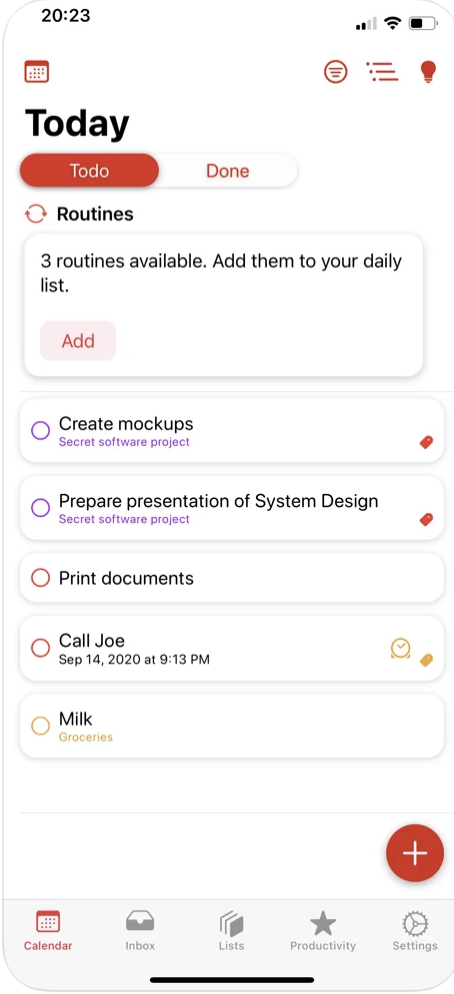
\includegraphics[width=4cm]{./graphics/planny4.png}
	\caption{An image of the 'today' view in the application Planny4\cite{reutter_2020}.}
	\label{fig:planny4}
	
\end{figure}
	        
	        There are many valuable features available in this application, the best one being the assistant suggesting ways to create a productive day.  However, apart from that, there are no other distinguishing features in this application that make it any better than other similar applications in the App Store.  The application also requires a subscription to unlock all features, and so is not an ideal solution for users unable to pay, such as students or low-income users.
	        
	        \subsection{24me - Smart Personal Assistant}
	        
	        24me\cite{24me} is an application available on iPhone, iPad and Apple Watch only and is mainly sold as a personal assistant more than a to-do or time management application.  Tasks can be viewed in a calendar (Figure~\ref{fig:24me}) or as a list, including reminders and labels.  The application also offers a way to automatically dial into conference calls, as well as Outlook email account integration and estimated times to get from one place to another.
	        
	        \begin{figure}[htb]

	\centering
	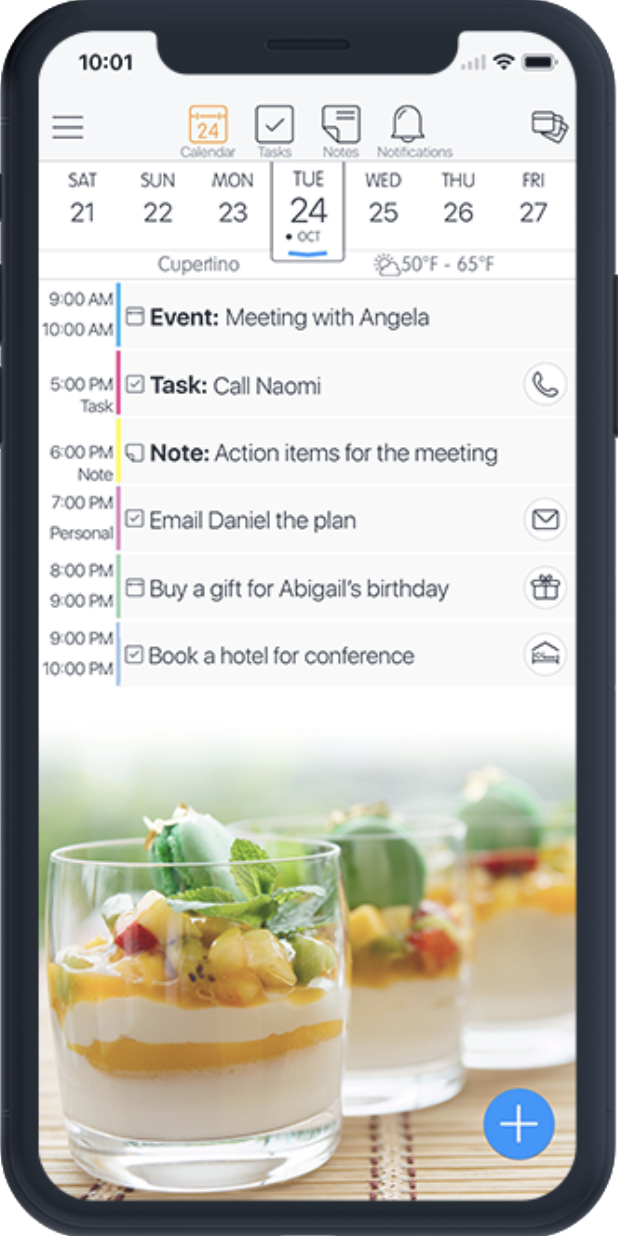
\includegraphics[width=4cm]{./graphics/24me.png}
	\caption{An image of the calendar view of the application 24me\cite{24me}.}
	\label{fig:24me}
	
\end{figure}
	        
	        This application has many unique features that are not seen in other productivity applications, such as conference calling and micro gifting, but the most basic features seem to need refinement.  Tasks cannot be customised much, and the UI, in general, seems to require some modernisation in order for this application to be a genuine competitor to other applications on the market.

	        \subsection{Any.do - Calendar and Reminders}
	        
	        Any.do\cite{any.do} is available on many different platforms, including Apple, Android, Windows and smart home devices.  The application allows users to create lists, view calendars, reminders and includes a daily planner.  Natural language processing is used to cherry-pick dates, times and location from reminders to make suggestions based on these items.  There are also extra features available on the premium version, including recurring, WhatsApp and location reminders, tags, themes and an unlimited daily planner.
	        
	        \begin{figure}[htb]

	\centering
	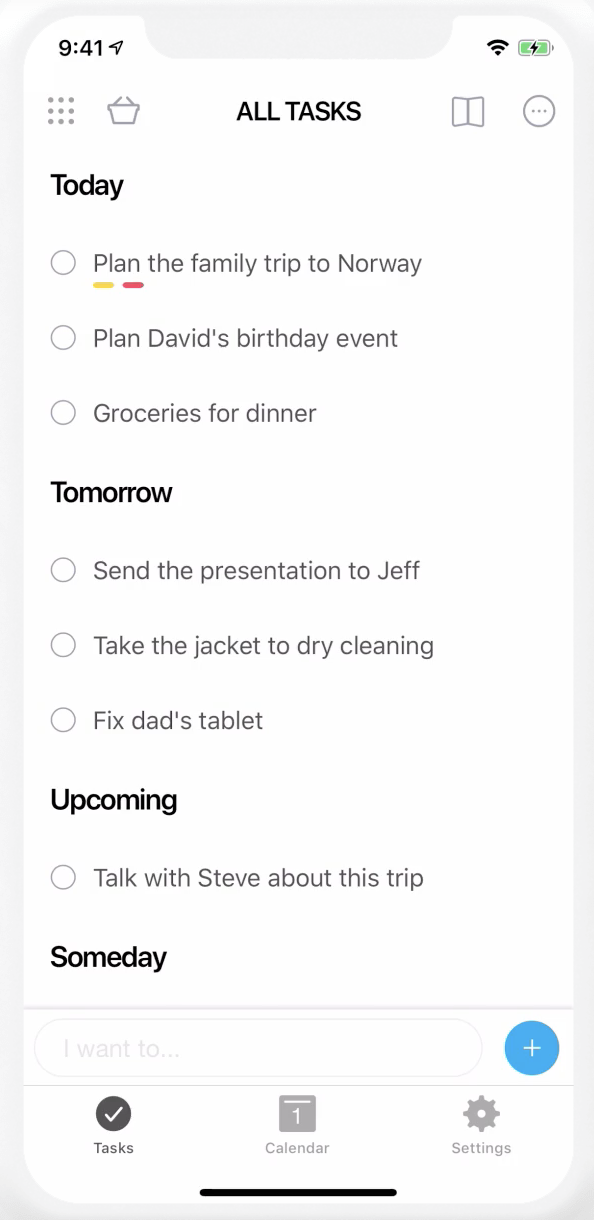
\includegraphics[width=4cm]{./graphics/anydo.png}
	\caption{An image of the task list view in the application any.do\cite{any.do}.}
	\label{fig:anydo}
	
\end{figure}
	        
	        Although this application does not necessarily boast any particularly unique features, the way the features have been implemented is elegant, making the application seem enjoyable to use and not too time-consuming for the user.  Tasks and reminders can be reordered easily, and the natural language processing features make creating new reminders a lot more efficient, which emphasises the purpose of the entire application.  However, it does seem incomplete without access to the premium features, which would be expected in a basic time management application, such as the tags and recurring reminders.
	        
	        \subsection{Things 3}
	        
	        Things 3\cite{things_3} is a paid application that allows users to create 'areas' to represent different parts of their life.  Within the 'areas', the user can create projects and plans that include to-do items and reminders, calendar integration, tags, and 'quick find'.  The application is available on all Apple platforms and synchronises all user data between these devices if the user is signed in on more than one device.
	        
	        \begin{figure}[htb]

	\centering
	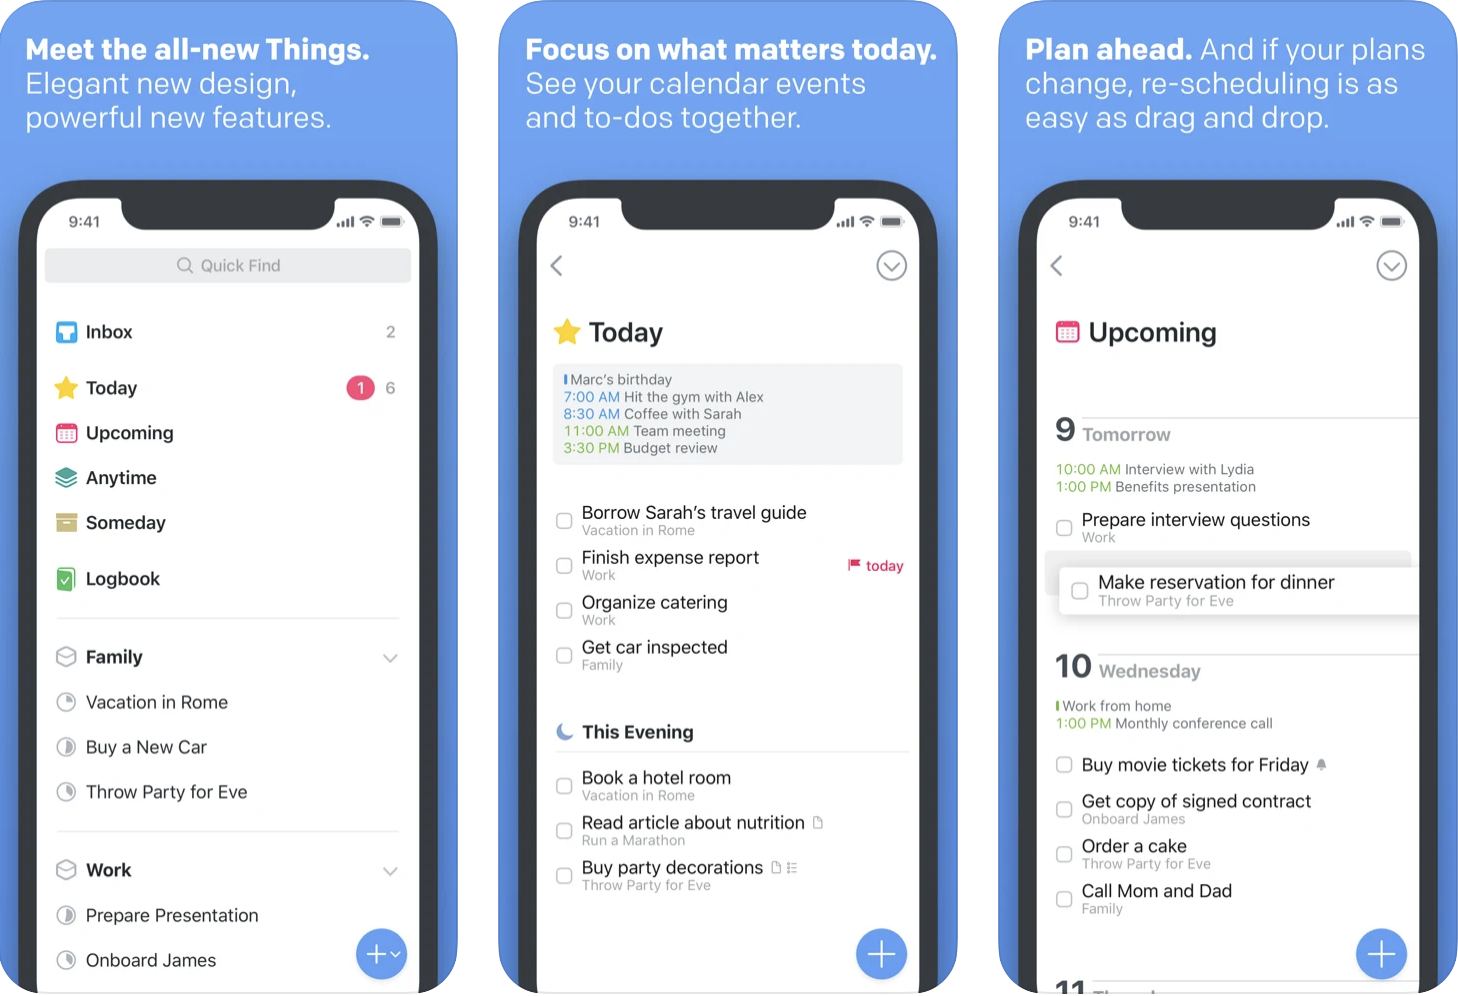
\includegraphics[width=10cm]{./graphics/things3.png}
	\caption{An image showing 'areas', today and this evening tasks and upcoming tasks in the application Things 3\cite{things_3}.}
	\label{fig:things3}
	
\end{figure}
	        
	        The main selling point for this application is that it allows the user to manage their time very precisely and do this for multiple areas of their life.  The 'areas' feature completely separates a users' career from their personal life for example.  Because of this, it is quite a strong competitor in the productivity application market.  The downside of this application is that the user must pay to download it; there is no free version or trial for the application to be tested, which can deter users from even trying the application. However, this can also be viewed positively. A subscription is not required to use the application. It is just a one-off payment, so if the user intends to use the application in the long term, it may be a worthwhile investment.
	        
	        \subsection{Sorted3}
	        
	        Sorted3\cite{sorted} is an application designed for 'hyper-scheduling' a users day.  It does this by putting all user events and tasks into a single unified timeline, so an entire day's outlook can be displayed.  The user can also tap on an event or task and add more detailed notes within the item to be referred back to if needed.  These notes can include a to-do list, tags and reminders for extra flexibility.  Features also include a timeline view, 'magic selection' of items so multiple can be selected at once, as well as natural language processing and Siri integration.
	        
	        \begin{figure}[htb]

	\centering
	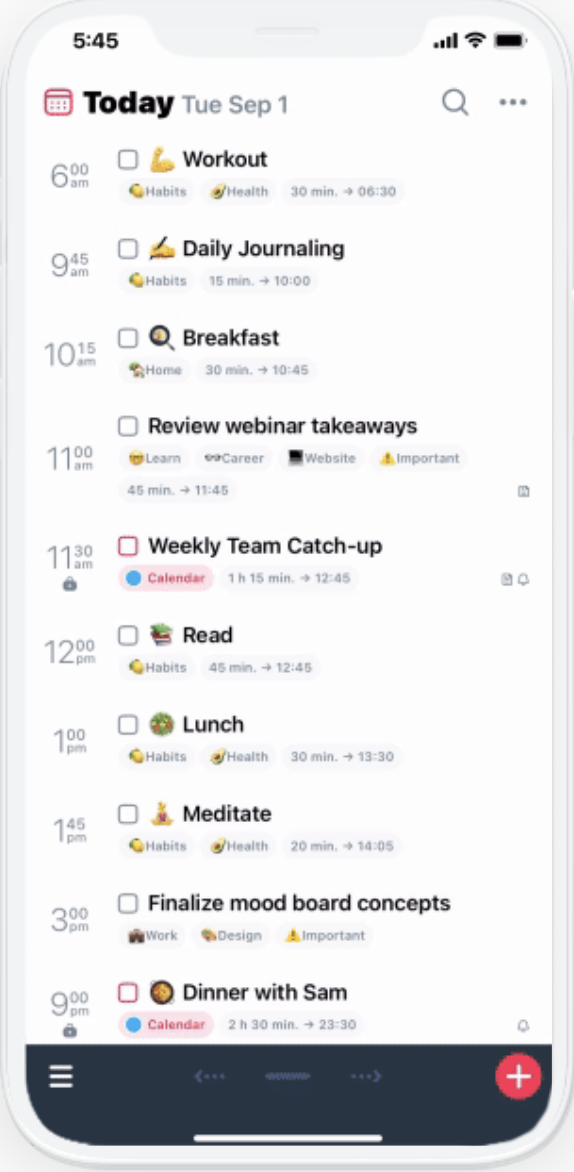
\includegraphics[width=4cm]{./graphics/sorted3.png}
	\caption{An image of the unified timeline feature withint the application Sorted3\cite{sorted}.}
	\label{fig:sorted3}
	
\end{figure}
	        
	        The most significant advantage of this application is that it gives users access to features expected to be part of the premium features.  For example, the unified timeline is quite a powerful feature considering it allows the user to view a complete overview of their day and add extreme detail to the items in the timeline if needed.  It also stands out from its competitors with features such as the 'magic selection' tool and the time ruler and calendar drawer.  There does not seem to be any other applications that offer these specific features, making Sorted 3 seem a much more elegant and well thought out choice.  As with many other applications, there are features only available with the premium option, including auto-scheduling and adding attachments to items.  However, the premium option is on a pay-once basis and offers features that are not necessarily considered compulsory for a productivity application.
	        
	        \subsection{OmniFocus 3}
	        
	        OmniFocus 3\cite{OmniFocus} is an application based on task management that users can use to create projects and add actions to them.  Various tags can be added to actions such as location, energy level and priority.  The perspectives view can help the user plan their day by seeing the subsequent actions that need to be completed.  A pro version allows the user to view a custom home screen and sidebar, a forecast tag, and custom perspectives.  This application is only available on Apple platforms or as a web application.
	        
	        \begin{figure}[htb]

	\centering
	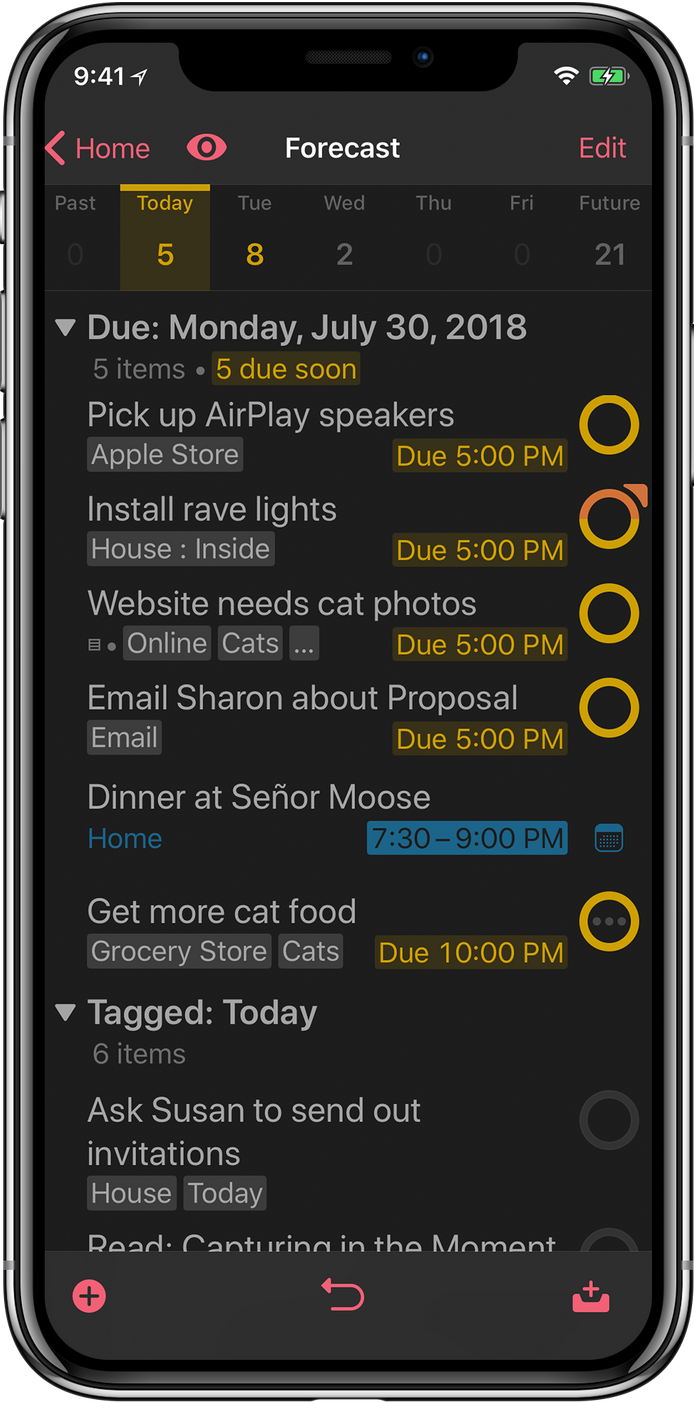
\includegraphics[width=4cm]{./graphics/omnifocus3.png}
	\caption{An image of the custom forecast tag within the pro version of the application Omnifocus\cite{OmniFocus}.}
	\label{fig:omnifocus3}
	
\end{figure}
	        
	        This application has many useful features but no features that particularly stand out against the other task management applications on the market.  The flexible tag management makes organising and batching actions a more intuitive process, and the perspectives view is also an excellent tool to allow the user the manage their time.  The features offered at a premium for the application are limited, especially as the price for premium access seems to be higher than the average. However, the user is offered two ways to pay for premium; a one-off payment that gives access to the iOS application only or a subscription that gives access to all platforms.
	        
	        \subsection{Related Work Summary}
	        
	        After taking into account the features available on various pre-existing productivity applications, it has been determined that the following features are considered indispensable for this application:
	        \begin{itemize}[noitemsep]
	            \item Creation of tasks, events and reminders.
	            \item Auto-scheduling.
	            \item Completely free access to the application.
	        \end{itemize}
	        
	        As discussed later in the document, Agendum has provided these features and other features which are highlighted in the requirements analysis.